\begin{frame}{Billiard Trajectories \href{https://youtu.be/A7mPzrNJHkA}{[video]}}
\begin{figure}
    \includegraphics[height=.8\textheight]{pics/1000_billiard_trajectories.pdf}
\end{figure}
\end{frame}

\begin{frame}{Integrability \& Conservation}
\begin{figure}
\includegraphics[height=.6\textheight]{pics/0000_integrability.png}
\end{figure}

\vspace*{-1cm}
\begin{align*}
\mbox{Energy} \implies L&=const.\\
\mbox{Joachmisthal's} \implies \gamma&=\frac{1}{2}\hat{v}.\nabla{f}(P)=const.
\end{align*}

\end{frame}

%\begin{frame}{Conservation: $L$ and $\gamma$}
%\begin{eqnarray*}
%f(x,y)&=&\left(\frac{x}{a}\right)^2+\left(\frac{y}{b}\right)^2=1 \\[10pt]
%\nabla{f}&=&2\left[\frac{x}{a^2},\frac{y}{b^2}\right]^t \\[10pt]
%\gamma&=&\frac{1}{2}\hat{v}.\nabla{f}(P)=\mbox{constant} >0,\,\,\,\forall{P}
%\end{eqnarray*}
%\end{frame}

\begin{frame}{$N=3$ Caustic \href{https://youtu.be/Y3q35DObfZU}{[video]}}
\begin{figure}
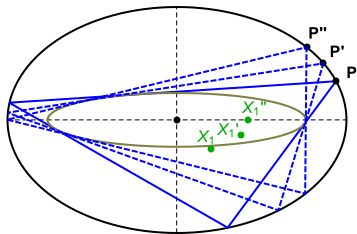
\includegraphics[height=.7\textheight]{pics/0010_three_orbits.pdf}
\end{figure}
\end{frame}

\begin{frame}{Poncelet's Porism}
\begin{figure}
    \centering
    \includegraphics[width=\textwidth]{pics/0003_poncelet_porism.pdf}
\end{figure}
\end{frame}

